\documentclass{article}
\usepackage{geometry}
\usepackage{amsmath}
\usepackage{amsfonts}
\usepackage{amssymb}
\usepackage{amsthm}
\usepackage{parskip}
\usepackage{multicol}
\usepackage{xcolor}
\usepackage{fancyhdr}
\usepackage{physics}
\usepackage{graphicx} % Required for inserting images
\usepackage{hyperref}
\usepackage{enumitem}
\usepackage{mathtools}

% commands
\newcommand{\deq}{\vcentcolon=}
\newcommand{\idd}{\text{đ}}
\newcommand{\nimplies}{\centernot\implies}
\newcommand{\vc}[1]{\boldsymbol{#1}}

% margin settings
\geometry{
    a4paper,
    left=7mm,
    right=7mm,
    top=2cm,
    bottom=7mm
}

% testing
\usepackage{blindtext}

% proof environments
\newtheorem{definition}{Definition}[section]
\newtheorem{theorem}{Theorem}[section]
\newtheorem{corollary}{Corollary}[theorem]
\newtheorem{lemma}[theorem]{Lemma}
\newtheorem*{remark}{Remark} % unnumbered remarks

% header and footer
\pagestyle{fancy}
\fancyfoot{} % removes footer
\fancyhf{}
\renewcommand{\headrulewidth}{0.5pt}
\fancyhead[L]{Honours complex variables}
\fancyhead[R]{\thepage}

\begin{document}

\begin{multicols*}{3}
% starred environment ensures text remains in same column
\noindent

\subsubsection*{D1.1.1: Complex numbers}
Let $z=x+iy$ and $w=a+ib$ where $x,y,a,b\in\mathbb{R}$.
Then $z$ and $w$ are complex numbers. Furthermore:
\begin{enumerate}
    \item $z=w$ \textbf{if{}f} $x=a$ and $y=b$.
    
    \item $\Re(z)\deq x$ and $\Im(z)\deq y$.
    
    \item $|z|\deq\sqrt{x^2+y^2}$
    
    \item The \textbf{complex conjugate} of $z$ is:
    $$\overline{z}\deq x-iy.$$

    \item Addition and multiplication:
    $$(x+iy)+(a+ib)=(x+a)+i(y+b)$$
    $$(x+iy)(a+ib)=(xa-yb)+i(xb+ya).$$

    \item $\mathbb{C}\deq\{x+iy:x,y\in\mathbb{R}\}$
\end{enumerate}
with rule $i^2=-1$.

\subsubsection*{L1.1.3}
Let $u,w,z\in\mathbb{C}$ where $z=x+iy$. Then:
\begin{enumerate}
    \item $z+w=w+z$ and $zw=wz$.
    
    \item $u+(z+w)=(u+z)+w$
    
    \item $u(zw)=(uz)w$
    
    \item $u(z+w)=uz+uw$
    
    \item $z+0=z$ and $1z=z$.
    
    \item $\exists\bigl(-z\deq-x+i(-y)\bigr)$:
    $z+(-z)=0$.

    \item $\exists z^{-1}: zz^{-1}=1$ where:
    $$z^{-1}\deq\frac{x}{x^2+y^2}+i\frac{-y}{x^2+y^2}.$$
\end{enumerate}

\subsubsection*{D1.1.5 and D1.1.7: Polar form}
Let $z\in\mathbb{C}$ and $z=x+iy$. Then:
\begin{align*}
    z
    &=r(\cos\theta+i\sin\theta) \\
    &=re^{i\theta}
\end{align*}
for $r=\sqrt{x^2+y^2}$ in complex plane.
\begin{center}
    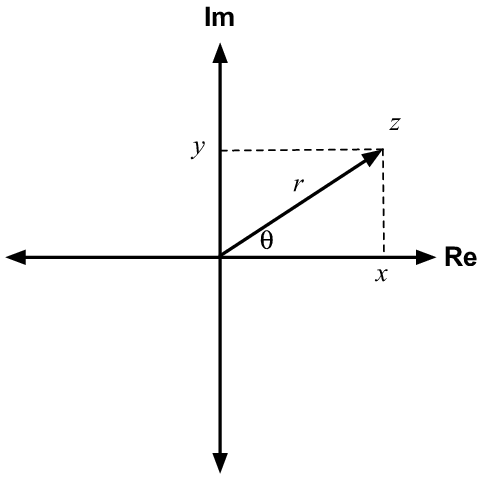
\includegraphics[scale=0.2]{f0.png}
\end{center}

\subsubsection*{L1.1.6}
Let $\theta,\phi\in\mathbb{R}$ and $n\in\mathbb{Z}$. Then:
\begin{enumerate}
    \item $e^{i(\theta+\phi)}=e^{i\theta}e^{i\phi}$
    
    \item $e^{in\theta}=(e^{i\theta})^n$
\end{enumerate}
due to de Moivre's formula:
$$\cos n\theta+i\sin n\theta=(\cos \theta+i\sin \theta)^n.$$

\newcolumn

\subsubsection*{L1.1.9}
Let $z,w\in\mathbb{C}$. Then:
\begin{enumerate}
    \item $|z|=0$ \textbf{if{}f} $z=0$.
    
    \item $|\overline{z}|=|z|$
    
    \item $|zw|=|z||w|$
    
    \item $\overline{\overline{z}}=z$
    
    \item $|z|^2=z\overline{z}$
    
    \item $\overline{z+w}=\overline{z}+\overline{w}$
    
    \item $\overline{zw}=\overline{z}\hspace{0.02in}\overline{w}$
    
    \item $|\Re(z)|\leq|z|$ and $|\Im(z)|\leq|z|$.
    
    \item $\Re(z)=\frac{1}{2}(z+\overline{z})$
    
    \item $\Im(z)=\frac{1}{2i}(z-\overline{z})$.
\end{enumerate}

\subsubsection*{L1.1.10 -- 11: Triangle inequalities}
Let $z,w\in\mathbb{C}$. Then:
\begin{enumerate}
    \item $|z+w|\leq|z|+|w|$
    
    \item $||z|-|w||\leq|z-w|$.
\end{enumerate}

\subsubsection*{D1.1.12: Argument of $z$}
Let $z=|z|e^{i\theta}$. Then:
$$\arg(z)\deq\theta\in(-\pi,\pi]$$
with period $2\pi$.

\subsubsection*{P1.1.14}
Let $z,w\in\mathbb{C}$. Then:
\begin{enumerate}
    \item $\arg(zw)=\arg(z)+\arg(w)$
    
    \item $\arg(\overline{z})=-\arg(z)$
\end{enumerate}
and holds under modulo $2\pi$.

\subsubsection*{D1.2.1: Open and closed $\epsilon$-discs}
Let $z_0\in\mathbb{C}$ and $\epsilon>0$.
\begin{enumerate}
    \item An \textbf{open} $\epsilon$-disc
    centred at $z_0$ is:
    $$D_{\epsilon}(z_0)
    \deq\{z\in\mathbb{C}:|z-z_0|<\epsilon\}.$$

    \item A \textbf{closed} $\epsilon$-disc
    centred at $z_0$ is:
    $$\overline{D}_{\epsilon}(z_0)
    \deq\{z\in\mathbb{C}:|z-z_0|\leq\epsilon\}.$$
\end{enumerate}
A \textbf{punctured} $\epsilon$-disc centred at $z_0$ is:
$$D'_{\epsilon}(z_0)\deq\{z\in\mathbb{C}:0<|z-z_0|<\epsilon\}.$$

\subsubsection*{D1.2.2: Open sets}
Let $U\subset\mathbb{C}$. Set $U$ is \textbf{open} if:
$$\forall z_0\in U;\exists\epsilon>0:D_{\epsilon}(z_0)\subseteq U.$$
Subset $F$ is \textbf{closed} if
$\mathbb{C}\hspace{0.02in}\backslash\hspace{0.02in} F$ is open.

A \textbf{neighbourhood} of point $z_0\in\mathbb{C}$
is an open set that contains $z_0$.

\subsubsection*{L1.2.3}
Punctured disc $D'_{\epsilon}(z_0)$ is open.

\subsubsection*{D1.2.4: Limit points}
Let $S\subseteq\mathbb{C}$. $z_0$ is a \textbf{limit point} of $S$ if:
$$\forall\epsilon>0; D'_{\epsilon}(z_0)\cap S\neq\emptyset.$$
The \textbf{closure} of $S$ is set $\overline{S}$ and contains $S$
and \textbf{all} its limit points.

\subsubsection*{L1.2.6}
Let $S\subseteq\mathbb{C}$.
$S$ is closed \textbf{if{}f} $S=\overline{S}$.

\subsubsection*{D1.2.7: Bounded sets}
Let $S\subseteq\mathbb{C}$. Set $S$ is \textbf{bounded} if:
$$\forall z\in S;\exists M>0:|z|\leq S.$$

\subsubsection*{D1.2.8: $\epsilon$-N convergence}
Let $\mathbb{N}=\{0,1,2,\dots\}$.

Let $(z_n)_{n\in\mathbb{N}}\subseteq\mathbb{C}$ be a sequence
and $z\in\mathbb{C}$.
Then $\displaystyle\lim_{n\rightarrow\infty}z_n=z$ if:
\begin{align*}
    &\forall\epsilon>0;\exists N\in\mathbb{N}:\forall n\geq N \\
    &\implies |z_n-z|<\epsilon.
\end{align*}

\subsubsection*{L1.2.9}
Let $z_n,z\in\mathbb{C}$ where $z_n=a_n+i b_n$.

Then $\displaystyle\lim_{n\rightarrow\infty}z_n=z$ \textbf{if{}f}:
$$\Re(z)=\lim_{n\rightarrow\infty}a_n
\hspace{0.05in}\text{and}\hspace{0.05in}
\Im(z)=\lim_{n\rightarrow\infty}b_n.$$

\subsubsection*{L1.2.10}
Let $S\subseteq\mathbb{C}$ and $z\in\mathbb{C}$.
Then $z\in\overline{S}$ \textbf{if{}f}:
$$\exists z_n\in S: z=\lim_{n\rightarrow\infty}z_n.$$

\subsubsection*{D1.2.11: Cauchy sequences}
$z_n$ is a Cauchy sequence if:
\begin{align*}
    &\forall\epsilon>0;\exists N\in\mathbb{N}:
    \forall n,m\geq N \\
    &\implies |z_n-z_m|<\epsilon.
\end{align*}

\subsubsection*{L1.2.12}
$z_n$ is convergent \textbf{if{}f} $z_n$ is Cauchy.

\subsubsection*{D1.2.14: Bounded sequences}
$z_n$ is bounded if:
$$\forall n\in\mathbb{N};\exists M>0:|z_n|\leq M.$$

\subsubsection*{L1.2.15: Bolzano-Weierstrass}
Let $z_n$ be a bounded sequence. Then:
$$\exists (z_{n_k})_{k,n_k\in\mathbb{N}}:
\lim_{k\rightarrow\infty}z_{n_k}=z\in\mathbb{C}$$
or that $z_n$ has a convergent subsequence.

A selection of a sequence is a subsequence.

\newcolumn

\subsubsection*{D1.3.1: Bounded functions}
Let $S\subseteq\mathbb{C}$ and $f:S\rightarrow\mathbb{C}$.
Then $f$ is a bounded function if:
$$\forall z\in S;\exists M>0:|f(z)|\leq M.$$

\subsubsection*{D1.3.2: $\epsilon$-$\delta$ convergence}
Let $S\subseteq\mathbb{C}, z_0\in\overline{S},f:S\rightarrow\mathbb{C}$
and $a_0\in\mathbb{C}$.
Then $\displaystyle\lim_{z\rightarrow z_0}f(z)=a_0$ if:
\begin{align*}
    &\forall z\in S;\forall\epsilon>0;\exists\delta>0:
    0<|z-z_0|<\delta \\
    &\implies|f(z)-a_0|<\epsilon.
\end{align*}

\subsubsection*{L1.3.3}
Let $S\subseteq\mathbb{C}, z_0\in\overline{S},
f:S\rightarrow\mathbb{C}$ and $a_0\in\mathbb{C}$ where $z_0=x_0+iy_0$
and $f=u+iv$.

Then $\displaystyle\lim_{z\rightarrow z_0}f(z)=a_0$ \textbf{if{}f}:
$$\Re(a_0)=\lim\limits_{\substack{
    x \to x_0 \\
    y \to y_0}}u(x,y)$$
and
$$\Im(a_0)=\lim\limits_{\substack{
    x \to x_0 \\
    y \to y_0}}v(x,y).$$

\subsubsection*{L1.3.4}
Let $S\subseteq\mathbb{C}, z_0\in\overline{S},
f:S\rightarrow\mathbb{C},a_0\in\mathbb{C}$ and sequence
$w_n\in S\hspace{0.02in}\backslash\hspace{0.02in}\{z_0\}$.

If $\displaystyle\lim_{z\rightarrow z_0}f(z)=a_0$
and $\displaystyle\lim_{n\rightarrow\infty}w_n=z_0$
then:
$$\lim_{n\rightarrow\infty}f(w_n)=a_0.$$

\subsubsection*{L1.3.5: Limit identities}
Let $S\subseteq\mathbb{C}, z_0\in\overline{S}$ and $a_0,b_0\in\mathbb{C}$. \\
Let $f,g:S\rightarrow\mathbb{C}$.

If $\displaystyle\lim_{z\rightarrow z_0}f(z)=a_0$
and $\displaystyle\lim_{z\rightarrow z_0}g(z)=b_0$
then:
\begin{enumerate}
    \item $\displaystyle\lim_{z\rightarrow z_0}
    (f(z)+g(z))=a_0+b_0$

    \item $\displaystyle\lim_{z\rightarrow z_0}
    (f(z)g(z))=a_0 b_0$

    \item $\displaystyle\lim_{z\rightarrow z_0}
    \left(\frac{f(z)}{g(z)}\right)=\frac{a_0}{b_0}$
    if $b_0\neq0$.
\end{enumerate}

\subsubsection*{D1.3.6: $\epsilon$-$\delta$ continuity}
Let $S\subseteq\mathbb{C}, f:S\rightarrow\mathbb{C}$
and $z_0\in S$.
Then $f$ is continuous at $z_0$ if:
\begin{align*}
    &\forall z\in S;\forall\epsilon>0;\exists\delta>0:
    |z-z_0|<\delta \\
    &\implies|f(z)-f(z_0)|<\epsilon.
\end{align*}

\subsubsection*{L1.3.7}
Let $f:\mathbb{C}\rightarrow\mathbb{C}$ with rule $f=u+iv$
and $z_0=x_0+iy_0\in\mathbb{C}$.

Then $f$ is continuous at $z_0$ \textbf{if{}f}
$u$ and $v$ are continuous at $(x_0,y_0)$.

\subsubsection*{L1.3.8}
If $f,g:\mathbb{C}\rightarrow\mathbb{C}$
are continuous at $z_0$ then:
\begin{enumerate}
    \item $f+g$ is continuous at $z_0$.
    
    \item $fg$ is continuous at $z_0$.
    
    \item $f/g$ is continuous at $z_0$.
    ($g\neq0$)
\end{enumerate}

\subsubsection*{D: Image and preimage}
Let $f:X\rightarrow Y$ where $A\subseteq X$ and $B\subseteq Y$.
The image of $A$ is:
$$f(A)=\{f(x):x\in A\}$$
and the preimage of $B$ is:
$$f^{-1}(B)=\{x:f(x)\in B\}.$$

\subsubsection*{L1.3.9}
Let $U\subseteq\mathbb{C}$ be an open set.
$f:\mathbb{C}\rightarrow\mathbb{C}$ is continuous \textbf{if{}f}
$\forall U\subseteq\mathbb{C}; f^{-1}(U)$ is open
for $f^{-1}(U)=\{z\in\mathbb{C}:f(z)\in U\}$.

\subsubsection*{L1.3.10}
Let $f:S\rightarrow\mathbb{C}$ be continuous.
Let $S\subseteq\mathbb{C}$ be closed and bounded.

Then $f(S)$ is closed and bounded.

\subsubsection*{D1.4.1: Differentiability}
Let $z_0\in\mathbb{C}$ and $U$ a neighbourhood of $z_0$.
Let $f:U\rightarrow\mathbb{C}$. Then $f$ is differentiable at $z_0$ if
the following limit exists:
$$f'(z_0)\deq\lim_{z\rightarrow z_0}\frac{f(z)-f(z_0)}{z-z_0}.$$

\subsubsection*{L1.4.3}
Let $z_0\in\mathbb{C}$ and $U$ a neighbourhood of $z_0$.
If $f:U\rightarrow\mathbb{C}$ is differentiable at $z_0$ then
$f$ is continuous at $z_0$.

\subsubsection*{L1.4.4}
Let $z_0\in\mathbb{C}$ and $U$ a neighbourhood of $z_0$.
Let $f,g:U\rightarrow\mathbb{C}$ be differentiable at $z_0$.
Then $f+g$, $fg$ and $f/g$ (where $g(z_0)\neq0$)
are all differentiable at $z_0$.

\subsubsection*{L1.4.5: Chain rule}
Let $z_0\in\mathbb{C}$ and $U$ a neighbourhood of $z_0$.
Let $g:U\rightarrow\mathbb{C}$ be such that $g(U)$ is a neighbourhood
of $g(z_0)$. Assume that $g$ is differentiable at $z_0$
and $f$ is differentiable at $g(z_0)$. Then $f\circ g$
is differentiable at $z_0$:
$$(f\circ g)'(z_0)=f(g(z_0))g'(z_0).$$

\subsubsection*{T1.4.6: Cauchy-Riemann equations}
Let $z_0\in\mathbb{C}$ and $U$ a neighbourhood of $z_0$.
Let $f:U\rightarrow\mathbb{C}$ be differentiable at $z_0$. \\
Let $z_0=x_0+i y_0$ and $f=u+iv$. Then:
$$\frac{\partial u}{\partial x}(x_0,y_0)
=\frac{\partial v}{\partial y}(x_0,y_0)$$
$$\frac{\partial u}{\partial y}(x_0,y_0)
=-\frac{\partial v}{\partial x}(x_0,y_0).$$

\subsubsection*{T1.4.8}
Let $z_0\in\mathbb{C}$ and $U$ a neighbourhood of $z_0$
for $z_0=x_0+i y_0$. Let $f:U\rightarrow\mathbb{C}$ where $f=u+iv$.
Assume that real functions $u$ and $v$ are
continuously differentiable on a neighbourhood of $(x_0,y_0)$.

Then $f$ is differentiable at $z_0$.

\subsubsection*{Remark}
$f$ is continuously differentiable if its first derivatives
are continuous.

\subsubsection*{D1.4.9: Holomorphic functions}
$f$ is \textbf{holomorphic} at $z_0$ if there exists a neighbourhood
$U$ of $z_0$ such that $f$ is defined and differentiable.

\subsubsection*{D1.4.13: Harmonic equations}
$h(x,y)$ is harmonic if for
$\forall(x,y)\in\mathbb{R}^2$ it satisfies Laplace's equation:
$$\frac{\partial^2h}{\partial x^2}(x,y)+
\frac{\partial^2h}{\partial y^2}(x,y)=0.$$

\subsubsection*{L1.4.14}
Let $u(x,y),v(x,y)$ be twice continuously differentiable
and that $f(x+iy)=u+iy$ is holomorphic on $\mathbb{C}$.

Then $u$ and $v$ are harmonic.

\subsubsection*{D1.4.15: Harmonic conjugates}
Let $U\subseteq\mathbb{R}^2$ and
$u:U\rightarrow\mathbb{R}$ be harmonic.
Then harmonic function $v:U\rightarrow\mathbb{R}$ is a
\textbf{harmonic conjugate} of $u$ if complex function
$f=u+iv$ is holomorphic on $U$.

\newcolumn

\subsubsection*{D1.5.1: Polynomial degree}
Let $P:\mathbb{C}\rightarrow\mathbb{C}$ be a polynomial.
The \textbf{degree} of $P$ 
is the highest power of the variable in $P$,
denoted as $\deg(P)$.

\subsubsection*{L1.5.2}
Let $z_0\in\mathbb{C}$. Let complex functions $f$ and $g$ be
holomorphic at $z_0$. Then $f+g$, $fg$ and $f/g$ ($g\neq0$)
are holomorphic at $z_0$.

\subsubsection*{C1.5.3}
Let $N\in\mathbb{N}$ and $a_0,\dots,a_N\in\mathbb{C}$. \\
Let $\displaystyle P(z)=\sum_{n=0}^{N}a_n z^n$. \\
Then $P(z)$ is holomorphic on $\mathbb{C}$ and:
$$P'(z_0)=\sum_{n=1}^{N}na_n z_0^{n-1}.$$

\subsubsection*{L1.5.4}

\subsubsection*{D1.5.5: Rational functions}
Let $P,Q:\mathbb{C}\rightarrow\mathbb{C}$. \\
Then $R:\{z\in\mathbb{C}:Q(z)\neq0\}\rightarrow\mathbb{C}$
with $R(z)=P(z)/Q(z)$ is a rational function.

\subsubsection*{L1.5.7}
The rational function $R(z)=P(z)/Q(z)$
is holomorphic on $\{z\in\mathbb{C}:Q(z)\neq0\}$.

\subsubsection*{L1.5.8}
Let $U\subseteq\mathbb{C}$ be open.
Let $g$ be holomorphic on $U$ and $f$ be holomorphic on $g(U)$.

Then $f\circ g$ is holomorphic on $U$.

\subsubsection*{L1.5.10}

\newcolumn

\subsubsection*{D1.6.1: Exponential function}
The complex exponential function is a function defined as
$\exp:\mathbb{C}\rightarrow\mathbb{C}$ and rule:
$$\exp(z)\deq e^x(\cos y+i\sin y)$$
where $z=x+iy$.

\subsubsection*{P1.6.2}
Let $z,w\in\mathbb{C}$.
\begin{enumerate}
    \item $\exp(z)$ is holomorphic on $\mathbb{C}$.
    
    \item $\exp(z)=\exp'(z)$

    \item $\exp(z+w)=\exp(z)\exp(w)$
    
    \item $\exp(z+2\pi i)=\exp(z)$
\end{enumerate}

\subsubsection*{D1.6.6: Cosine and sine functions}
$$\cos(z)\deq\frac{1}{2}\Bigl(\exp(iz)+\exp(-iz)\Bigr)$$
$$\sin(z)\deq\frac{1}{2i}\Bigl(\exp(iz)-\exp(-iz)\Bigr)$$

\subsubsection*{L1.6.7}
Let $z\in\mathbb{C}$ where $z=x+iy$. Then:
\begin{enumerate}
    \item $\cos(z)$ and $\sin(z)$ are holomorphic at $z$,
    where $\cos'(z)=-\sin(z)$ and $\sin'(z)=\cos(z)$.

    \item $\cos^2(z)+\sin^2(z)=1$
    
    \item $\cos(z+2\pi)=\cos(z)$ \\
    $\sin(z+2\pi)=\sin(z)$
\end{enumerate}

\subsubsection*{L1.6.8}
Let $z,w\in\mathbb{C}$. Then:
\begin{enumerate}
    \item $\sin(z+\pi/2)=\cos(z)$
    
    \item $\sin(z+w) \\
    =\sin(z)\cos(w)+\sin(w)\cos(z)$

    \item $\cos(z+w) \\
    =\cos(z)\cos(w)-\sin(z)\sin(w)$.
\end{enumerate}

\subsubsection*{L1.6.9}
Let $z\in\mathbb{C}$ where $z=x+iy$. Then:
\begin{align*}
    &\sin(x+iy) \\
    &=\sin(x)\cosh(y)+i\cos(x)\sinh(y)
    \newline \\[0.025in]
    &\cos(x+iy) \\
    &=\cos(x)\cosh(y)-i\sin(x)\sinh(y).
\end{align*}

\subsubsection*{D1.6.11: Hyperbolic functions}
$$\cosh(z)\deq\frac{1}{2}\Bigl(\exp(z)+\exp(-z)\Bigr)$$
$$\sinh(z)\deq\frac{1}{2}\Bigl(\exp(z)-\exp(-z)\Bigr)$$

\subsubsection*{L1.6.12}
Let $z\in\mathbb{C}$. Then $\sinh(iz)=i\sin(z)$
and $\cosh(iz)=\cos(z)$.

\end{multicols*}

\end{document}